\documentclass{article}
\usepackage{amsmath,amssymb,amsthm,latexsym,paralist,url}
\usepackage[margin=1in]{geometry}
\usepackage{tikz}
\usetikzlibrary{arrows,automata}

\theoremstyle{definition}
\newtheorem{problem}{Problem}
\newtheorem*{solution}{Solution}
\newtheorem*{resources}{Resources}


\newcommand{\honor}{\noindent \textbf{Aggie Honor Statement: }On my honor as an Aggie, I have neither
  given nor received any unauthorized aid on any portion of the academic work included in this assignment.
}


\newcommand{\checklist}{\noindent\textbf{Checklist:}
Did you...
\begin{compactenum}
\item abide by the Aggie Honor Code?
\item solve all problems?
\item start a new page for each problem?
\item show your work clearly?
\item type your solution?
\item submit a PDF to eCampus?
\end{compactenum}
}

\newcommand{\problemset}[1]{\begin{center}\textbf{Problem Set #1}\end{center}}
\newcommand{\duedate}[1]{\begin{quote}\textbf{Due: #1} on eCampus (\url{ecampus.tamu.edu}). \\You must show your work in order to recieve credit.\end{quote}}
\newcommand{\mysectionnumber}[0]{503}

\title{CSCE 222: Discrete Structures for Computing\\Section \mysectionnumber\\Fall 2016}
\author{Joseph Martinsen}

\begin{document}

\maketitle

\problemset{8}

\duedate{23 October 2016 (Sunday) before 11:59 p.m.}

\bigskip

% Finite State Automata
\begin{problem} (30 points)\\
Find the language recognized by the given DFA:
\begin{enumerate}
\item \ \\
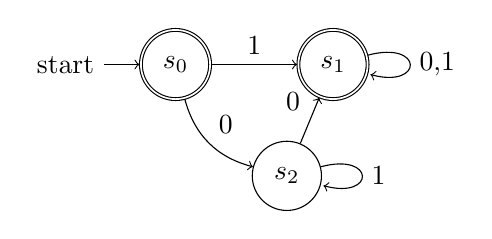
\begin{tikzpicture}[auto,node distance=2cm]
\node[initial,state,accepting] (s0) {$s_0$};
\node[state,accepting] (s1) [right of=s0] {$s_1$};
\node[state] (s2) [below right of=s0] {$s_2$};

\path[->]	(s0)	edge				node	{1}	(s1)
			edge	[bend right]	node	{0}	(s2)
		(s1)	edge	[loop right]	node	{0,1}	(s1)
		(s2) 	edge 				node	{0}	(s1)
		(s2) 	edge	[loop right] 	node	{1}	(s2);
\end{tikzpicture}
\item \ \\
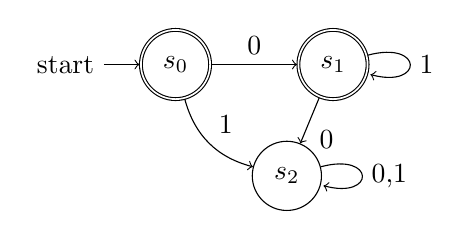
\begin{tikzpicture}[auto,node distance=2cm]
\node[initial,state,accepting] (s0) {$s_0$};
\node[state,accepting] (s1) [right of=s0] {$s_1$};
\node[state] (s2) [below right of=s0] {$s_2$};

\path[->]	(s0)	edge				node	{0}	(s1)
			edge	[bend right]	node	{1}	(s2)
		(s1)	edge	[loop right]	node	{1}	(s1)
			edge 				node	{0}	(s2)
		(s2) 	edge	[loop right] 	node	{0,1}	(s2);
\end{tikzpicture}
\item \ \\
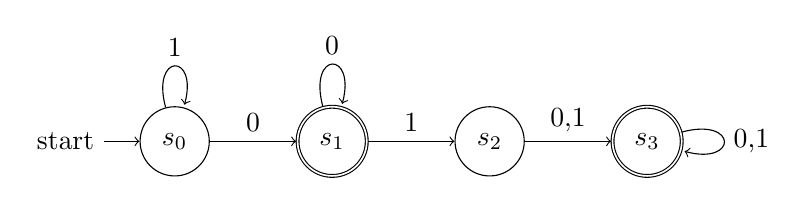
\begin{tikzpicture}[auto,node distance=2cm]
\node[initial,state] (s0) {$s_0$};
\node[state,accepting] (s1) [right of=s0] {$s_1$};
\node[state] (s2) [right of=s1] {$s_2$};
\node[state,accepting] (s3) [right of=s2] {$s_3$};

\path[->]	(s0)	edge				node	{0}	(s1)
			edge	[loop above]	node	{1}	(s0)
		(s1)	edge	[loop above]	node	{0}	(s1)
			edge				node	{1}	(s2)
		(s2) 	edge 				node	{0,1}	(s3)
		(s3) 	edge	[loop right] 	node	{0,1}	(s3);
\end{tikzpicture}
\end{enumerate}
\end{problem}

\begin{solution}\ \\
  \begin{enumerate}
    \item
    \begin{align*}
      (0,1)^{*} & \quad\text{From } s_1 \\
      \lambda & \quad \text{From } s_0 \\
      L(m) =& 1(0,1)^* \big| \lambda
    \end{align*}
    \item
    \begin{align*}
      1^{*} &\quad\text{from } s_2 \\
      \lambda &\quad \text{from } s_0 \\
      L(m) =&  01^* \mid \lambda
    \end{align*}
    \item
    \begin{align*}
      1^{*}0 \quad \text{from } s_0 \\
      0+ &\quad \text{from } s_1 \\
      (0,1)+ &\quad \text{from } s_3 \\
      L(m) =& 1^{*}0^{+} \mid 1^{*}0^{+}1(0,1)^+
    \end{align*}
  \end{enumerate}
\end{solution}

\newpage

% Grammars
\begin{problem} (20 points)\\
Show that the following grammar generates the language $\{a^nb^nc^n \mid n\geq 0\}$.
\begin{align*}
S &::= aST \mid \lambda\\
T &::= BC\\
CB &::= BC\\
aB &::= ab\\
bB &::= bb\\
bC &::= bc\\
cC &::= cc
\end{align*}
\end{problem}

\begin{solution}\ \\
  \begin{align}
    S ::= aST \mid \lambda \quad\quad&\text{from this it can be seen the case when } n=0 \text{ for } a,b,c \text{ is true. Also, if not }\\
    \quad\quad& \lambda \text{ the S string will continue to repeat itself thus the string must start with } a^n \\
    a^{n}B^{n}C^{n} \quad\quad&  \text{ from } T ::= BC\\
    %CB ::= BC \quad\quad& \\
    a^{n}b^{n}C^{n} \quad\quad& \text{from }aB ::= ab\\
    %bB ::= bb \quad\quad& \\
    a^{n}b^{n}c^{n}\quad\quad& \text{from }bC ::= bc 
    %cC ::= cc \quad\quad&
  %   \text{Another path is for when } &T::=CB \text{ from } CB::=BC \\
  %   a^{n}C^{n}B^{n} \quad\quad& \text{from lines } 1 \text{ and } 6
  % \end{align}
\end{solution}

\bigskip
\honor

\bigskip
\checklist
\end{document}
